\subsection{Listings}
% \begin{frame}[c,plain,noframenumbering]
% \begin{tikzpicture}[remember picture,overlay]
% \fill[fill=gray]
%     (current page.south east)  rectangle ([shift={(0,-0.1\paperheight)}]current page.north west)   ;
% \end{tikzpicture}
% \centering
% \vfill
% \textcolor{white}{\Large\textbf{Listings}}
% \end{frame}


\begin{frame}[fragile]{Inserting a Listing}
\vspace{.5cm}
	\begin{columns}[t]
		\begin{column}{.5\textwidth}
			Instead of pseudocode, you can also typeset actual code.
			This is called a \textit{listing}
			\begin{itemize}
			\item[] \pack{listings}
			\\\envs{lstlisting}{\\\quad\textless code here\textgreater\\}
			\end{itemize}
			\vskip.02\textheight
			Or input code file directly, using
			\\\commop{lstinputlisting}{language=\\programmingLanguage}{PathToSourcefile}
		\end{column}
		\begin{column}{.5\textwidth}
			The listings package supports many programming languages,
			but still enables you to customize everything you want
			\vskip.05\textheight
			Full explanation: \href{https://en.wikibooks.org/wiki/LaTeX/Source_Code_Listings}{https://en.wikibooks.org/wiki/\\LaTeX/Source\_Code\_Listings}
		\end{column}
	\end{columns}	
\end{frame}


\begin{frame}[fragile]{Inserting a Listing}
Actual listing and result
%\vspace{.5cm}
	\begin{columns}[t]
		\begin{column}{.5\textwidth}
			\begin{figure}
			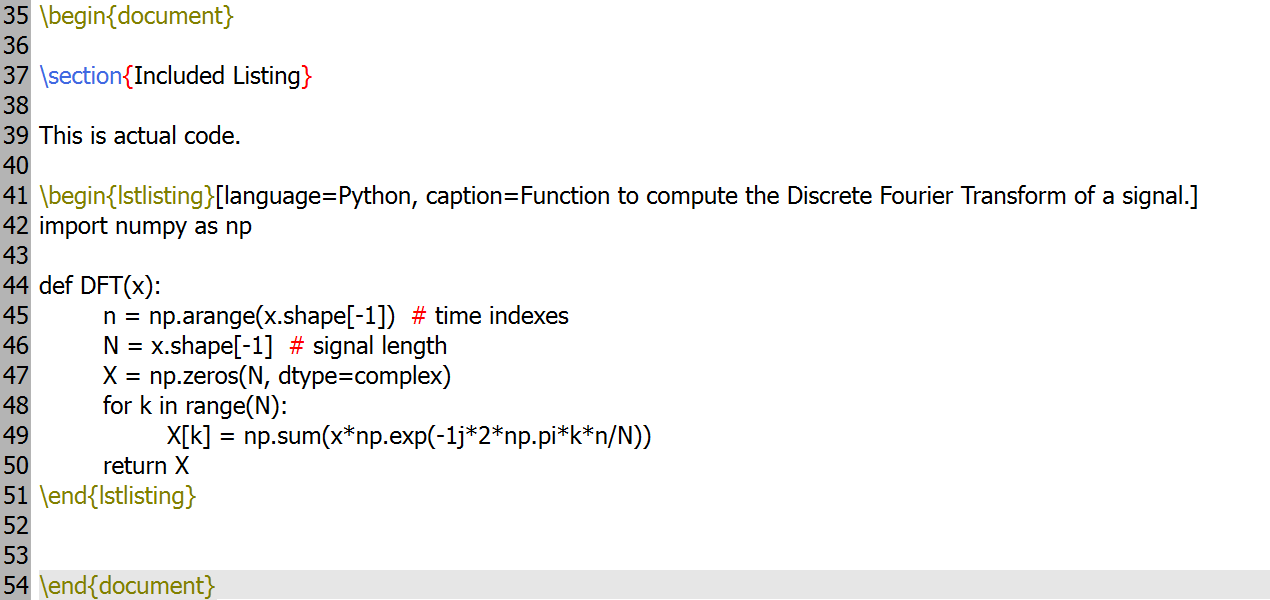
\includegraphics[scale=.35]{Figures/code6_2}
			\end{figure}
		\end{column}
		\begin{column}{.5\textwidth}
			\begin{figure}
			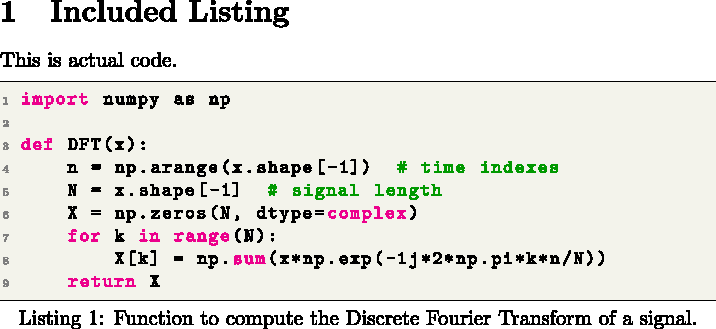
\includegraphics[width=.84\linewidth, frame, trim={-1cm -1cm -1cm -1cm},clip]{Figures/doc8}
			\end{figure}
		\end{column}
	\end{columns}
	\vskip.1\textheight
	Better package for Python: minted, \href{https://ctan.org/pkg/minted}{https://ctan.org/pkg/minted}
\end{frame}




\begin{frame}[fragile]{Code highlighting with minted}
\vspace{.5cm}
	\begin{columns}[t]
		\begin{column}{.6\textwidth}
            \begin{figure}
                \centering
                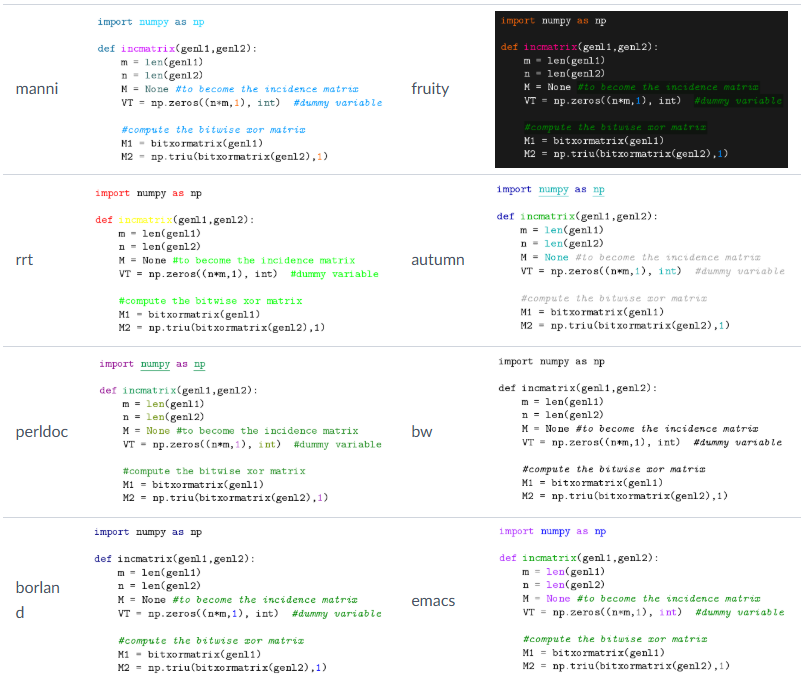
\includegraphics[width=\linewidth]{Figures/minted.png}
            \end{figure}
		\end{column} 
		\begin{column}{.4\textwidth}
			The minted package supports many programming languages, but requires installing Pygments. (supported out-of-the-box in Overleaf)
			\somespace
			More information: \url{https://www.overleaf.com/learn/latex/Code_Highlighting_with_minted}
		\end{column}
	\end{columns}	
\end{frame}

% \begin{frame}[fragile]{Inserting a Listing}
% Defining custom style
% %\vspace{.5cm}
% 	\begin{columns}[t]
% 		\begin{column}{.5\textwidth}
% 			\begin{figure}
% 			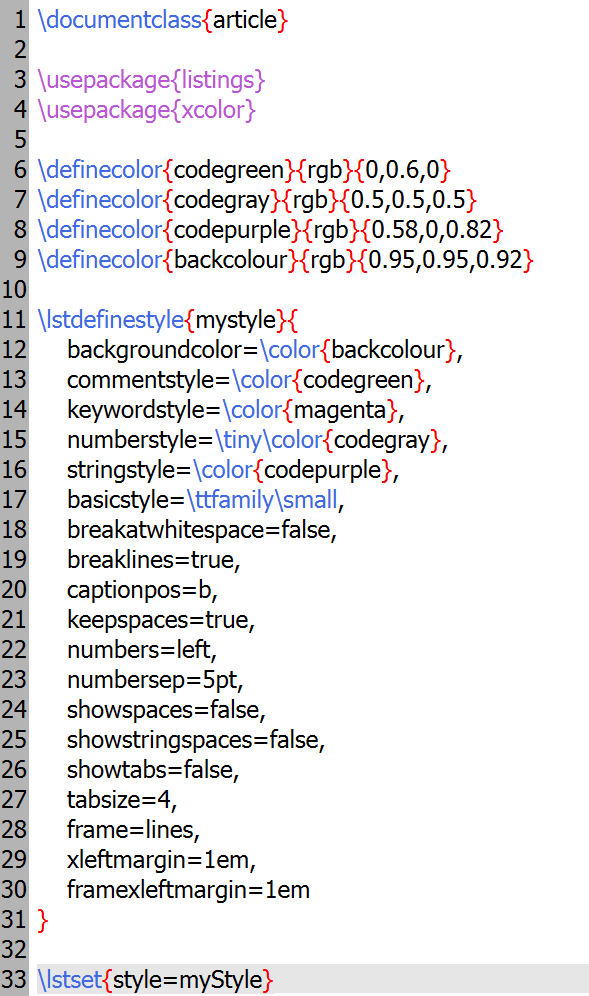
\includegraphics[scale=.35]{Figures/code6_1}
% 			\end{figure}
% 		\end{column}
% 		\begin{column}{.5\textwidth}
% 		\end{column}
% 	\end{columns}	
% \end{frame}
